\subsubsection{Ejercicio 1}

Sea $A(n)$ un número real tal que
\begin{equation}
A(n) = \sum_{n=1}^\infty \dfrac{1}{n}
\end{equation}
Se implementa una programa en Fortran que permite calcular y graficar $A(n)$ para ciertos valores de $n$. En la Figura \ref{fig_P1_1_1} se grafica $A$ para simple y doble precisión. En la Figura \ref{fig_P1_1_2} Para doble y cuadruple precisión

\begin{figure} [H]
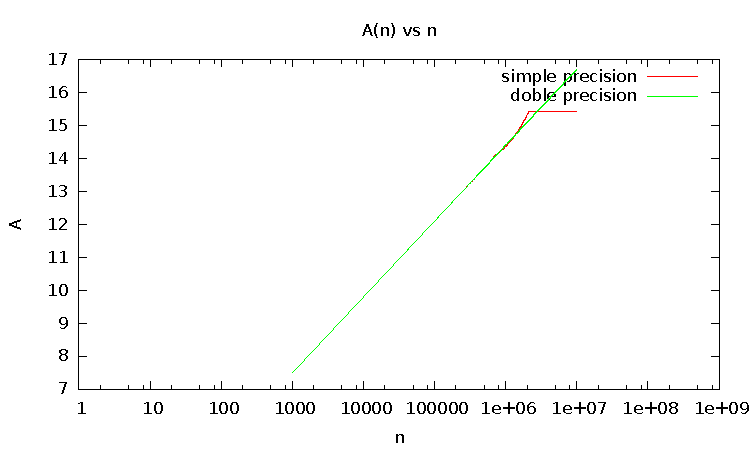
\includegraphics{./parte2/graficos/grafico_p1_1.pdf}
\caption{} \label{fig_P1_1_1}
\end{figure}

\begin{figure} [H]
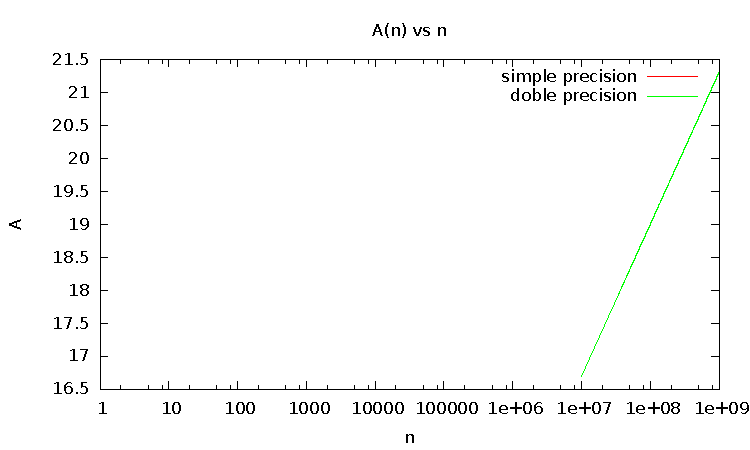
\includegraphics{./parte2/graficos/grafico_p1_2.pdf}
\caption{} \label{fig_P1_1_2}
\end{figure}

%----------------------------------------------
\subsubsection{Ejercicio 2}
Se implementa una rutina en Fortran que permite calcular los $n+1$ valores de la serie Fibonacci
\begin{equation}
u_{n+1} = u_{n} + u_{n-1} \hspace{1cm} \mbox{tal que} \hspace{0,5cm} u_0=0 \hspace{0,1cm} ; \hspace{0,1cm} u_1=1
\end{equation}
La serie se grafica para $n=100$

\begin{figure} [H]
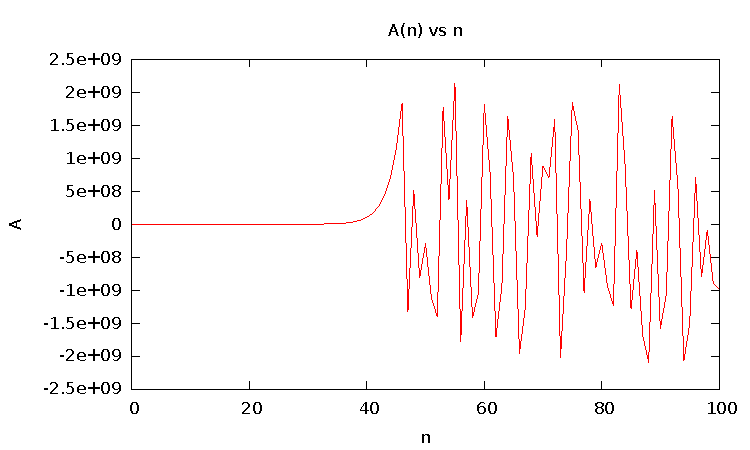
\includegraphics{./parte2/graficos/grafico_p2.pdf}
\caption{} \label{fig_P1_2}
\end{figure}